\renewcommand{\chaptername}{March 8th: Lab}
\chapter{Qubits and Quantum Circuits}

Conventionally, information is stored in bits, as a series of 0s and 1s. In quantum computing `quantum bits', or simply `qubits', are used. These obey the rules of quantum mechanics and allow for information to be processed in new and different ways.

In order to manipulate these qubits (i.e. change them between quantum states) `quantum gates' can be applied to build a 'quantum circuit'. A quantum circuit is a computational routine consisting of coherent quantum operations on quantum data, such as qubits, and concurrent real-time classical computation. It is an ordered sequence of quantum gates, measurements and resets, all of which may be conditioned on and use data from the real-time classical computation.

\section{Objectives}
The purpose of this lab is to investigate quantum bits and quantum circuits using IBM's `qiskit`. In this fashion, the following objectives were pursued:
\begin{itemize}
    \item Become familiar with `qiskit'
    \item Implement quantum gates and visualise the state of a qubit through the Bloch sphere
    \item Obtain deeper understanding of quantum operations and quantum circuits basics
\end{itemize}

\section{Methods}
Quantum circuits were implemented and visualised using python in Jupyter Notebook - a web-based interactive computational environment for programming languages. Specifically, a module named `qiskit' was used; an open-source software development kit (SDK) for working with quantum computers at the level of circuits, pulses, and algorithms. It provides tools for creating and manipulating quantum programs and running them on prototype quantum devices on IBM Quantum Experience or on simulators on a local computer. Qiskit is made up of elements that each work together to enable quantum computing. The Aer simulator provides high-performance quantum computing simulators with realistic noise models locally, and visualization allows you to see what you states look like

To evaluate the rigidity of the analytical predictions from qiskit, IBMs quantum computer was used. `The IBM Quantum Composer' is an online platform allowing public access to remote quantum computing services provided by IBM Quantum.

%Reference screenshots of code

\section{Results}
Qubits can be represented by 2D vectors, their states are limited to the form:

$$ |q\rangle = \cos{\tfrac{\theta}{2}}|0\rangle + e^{i\phi}\sin{\tfrac{\theta}{2}}|1\rangle $$
where $\theta$ and $\phi$ are real numbers. 

\subsection{The Pauli Gates}
An important feature of quantum circuits is that, between initialising the qubits and measuring them, the operations (gates) are *always* reversible! These reversible gates can be represented as matrices, and as rotations around the Bloch sphere. visualise the state of a qubit through the Bloch sphere.
Pauli matrices can represent some commonly used quantum gates.to manipulate the quantum states through the use of gates, the operations that change a qubit between states

\subsubsection{The X Gate}
The X-gate is represented by the Pauli-X matrix:

$$ X = \begin{bmatrix} 0 & 1 \\ 1 & 0 \end{bmatrix} = |0\rangle\langle1| + |1\rangle\langle0| $$

To see the effect an X gate has on a qubit, qiskit was used. A qubit was initialised in state $|0\rangle$ and was passed through an Pauli-X gate. The diagram for this circuit is shown in Figure \ref{fig:xGate}.

\begin{figure}[h]
    \centering
    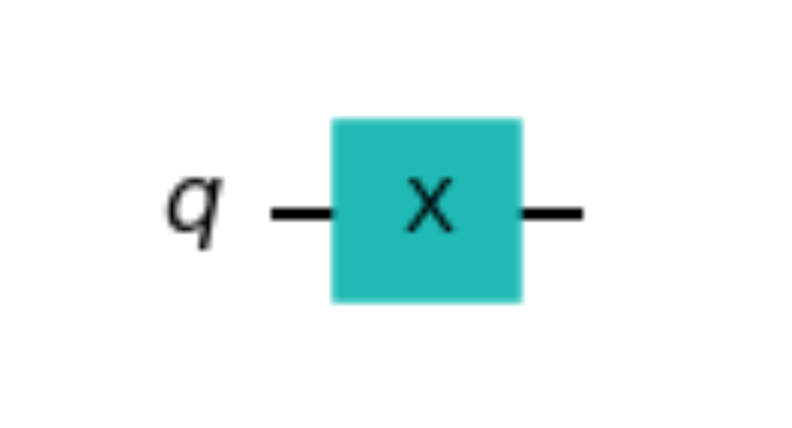
\includegraphics[width=0.3\textwidth]{lab2/images/xGate.png}
    \caption{Circuit Diagram of X gate applied to qubit} 
    \label{fig:xGate}
\end{figure}

From the mathematics, it is clear that applying an X-gate switches the amplitudes of the states $|0\rangle$ and $|1\rangle$:

$$ X|0\rangle = \begin{bmatrix} 0 & 1 \\ 1 & 0 \end{bmatrix}\begin{bmatrix} 1 \\ 0 \end{bmatrix} = \begin{bmatrix} 0 \\ 1 \end{bmatrix} = |1\rangle$$

This was demonstrated by observing the bloch sphere. Figure \ref{fig:bSphereXGate} shows the qubit has switched to state $|1\rangle$ after being initialised in state $|0\rangle$.

\begin{figure}[h]
    \centering
    \begin{subfigure}[h]{0.4\textwidth}
        \centering
        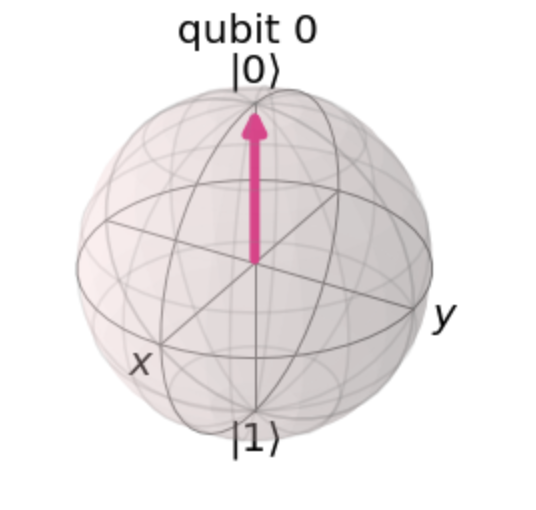
\includegraphics[width=\textwidth]{lab2/images/bSphX1.png}
        \caption{Bloch sphere showing the initialised qubit in state $|0\rangle$}
        \label{fig:bSphX1}
    \end{subfigure}
    \hfill
    \begin{subfigure}[h]{0.4\textwidth}
        \centering
        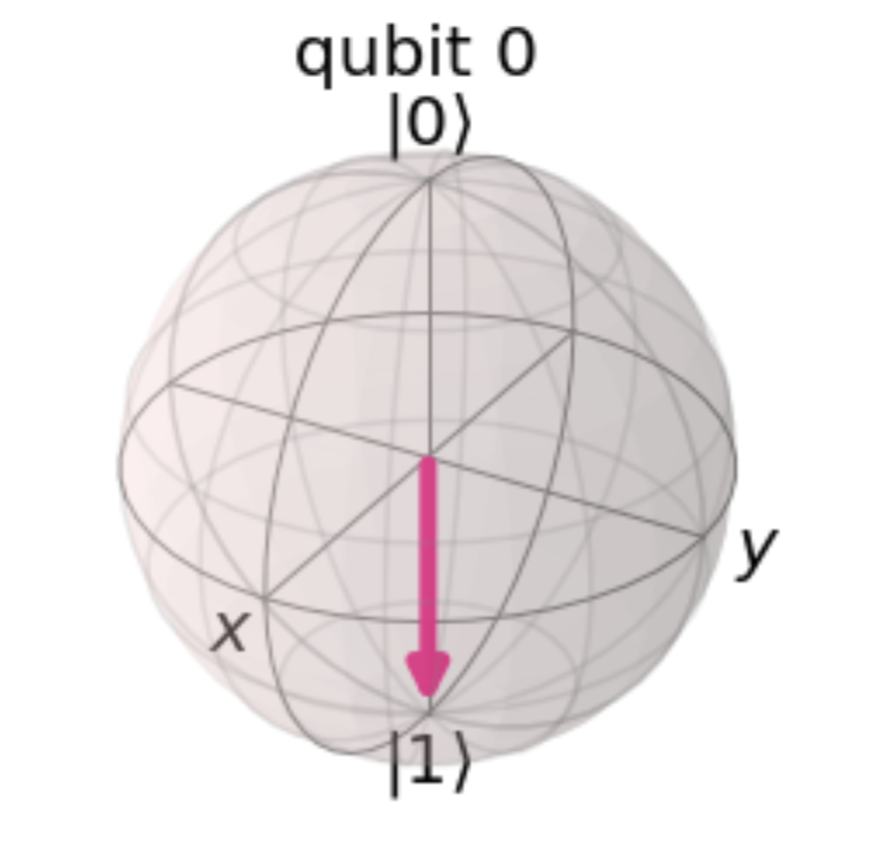
\includegraphics[width=\textwidth]{lab2/images/bSphX2.png}
        \caption{Bloch sphere showing the qubit in state $|1\rangle$ after being put through an X gate}
        \label{fig:bSphX2}
    \end{subfigure}
    \caption{Bloch sphere showing qubit state before and after X gate is applied} 
    \label{fig:bSphereXGate}
\end{figure}

\subsection{The Y and Z gates}


Similarly to the X-gate, the Y and Z Pauli matrices also act as the Y and Z-gates in our quantum circuits:


$$ Y = \begin{bmatrix} 0 & -i \\ i & 0 \end{bmatrix} = -i|0\rangle\langle1| + i|1\rangle\langle0| $$

$$ Z = \begin{bmatrix} 1 & 0 \\ 0 & -1 \end{bmatrix} = |0\rangle\langle0| - |1\rangle\langle1| $$

And, unsurprisingly, they also respectively perform rotations by $\pi$ around the y and z-axis of the Bloch sphere.

Figure \ref{fig:xyGateDiagram} shows the circuit diagram of a qubit with an X gate and a Y gate being applied to it%Bad GRAMMER

\begin{figure}[h]
    \centering
    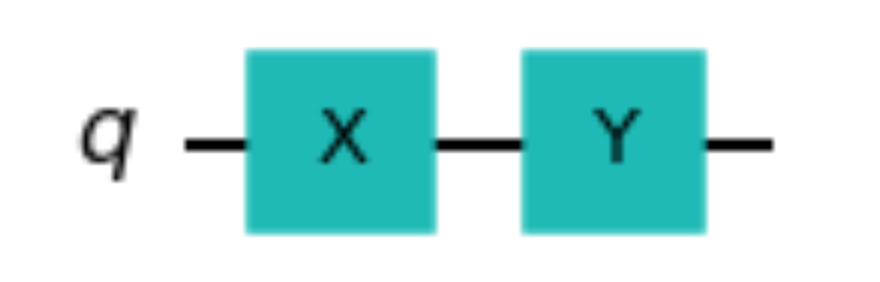
\includegraphics[width=0.3\textwidth]{lab2/images/xyGate.png}
    \caption{Circuit Diagram of X gate and Y gate applied to qubit} 
    \label{fig:xyGateDiagram}
\end{figure}

This results in the same as the start as seen in Figure \ref{fig:xyGateBloc}. The x gate rotates by $\pi$ around the x-axis, resulting in state $|1\rangle$. The y gate takes this resultant state and rotates it by $\pi$ around the y-axis, resulting in a qubit in state $|0\rangle$

\begin{figure}[h]
    \centering
    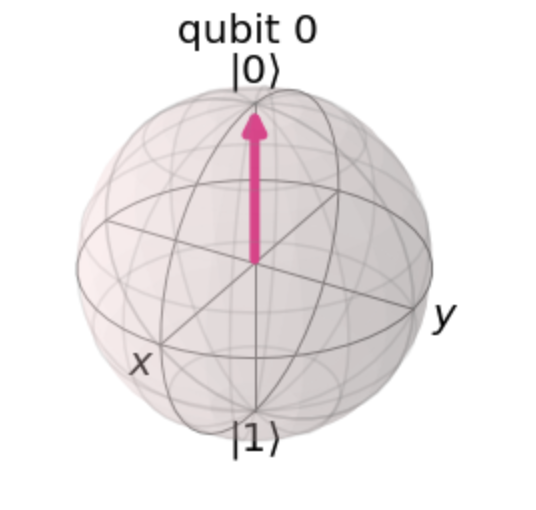
\includegraphics[width=0.5\textwidth]{lab2/images/bSphX1.png}
    \caption{X gate and Y gate applied to qubit, represented on a Bloch sphere} 
    \label{fig:xyGateBloc}
\end{figure}

\subsection{The Hadamard Gate}
The Hadamard gate (H-gate) is a fundamental quantum gate. It allows states to occupy a superposition of $|0\rangle$ and $|1\rangle$. It has the matrix:

$$ H = \tfrac{1}{\sqrt{2}}\begin{bmatrix} 1 & 1 \\ 1 & -1 \end{bmatrix} $$

We can see that this performs the transformations below:

$$ H|0\rangle = |+\rangle $$

$$ H|1\rangle = |-\rangle $$

This can be thought of as a rotation around the Bloch vector `[1,0,1]` (the line between the x and z-axis), or as transforming the state of the qubit between the X and Z bases.

Applying an x gate is the same as applying the sequence of gates, HZH, shown mathematically below:

$$ H = \tfrac{1}{\sqrt{2}}\begin{bmatrix} 1 & 1 \\ 1 & -1 \end{bmatrix} \quad\quad  Z = \begin{bmatrix} 1 & 0 \\ 0 & -1 \end{bmatrix} \quad\quad  X = \begin{bmatrix} 0 & 1 \\ 1 & 0 \end{bmatrix} $$

\begin{equation*} 
\begin{split}
HZH & = \tfrac{1}{\sqrt{2}}\begin{bmatrix} 1 & 1 \\ 1 & -1 \end{bmatrix} \begin{bmatrix} 1 & 0 \\ 0 & -1 \end{bmatrix}\tfrac{1}{\sqrt{2}}\begin{bmatrix} 1 & 1 \\ 1 & -1 \end{bmatrix} \\
HZH & = \tfrac{1}{\sqrt{2}}\tfrac{1}{\sqrt{2}}\begin{bmatrix} 1 & 1 \\ 1 & -1 \end{bmatrix} \begin{bmatrix} 1 & 0 \\ 0 & -1 \end{bmatrix}\begin{bmatrix} 1 & 1 \\ 1 & -1 \end{bmatrix} \\
HZH & = \tfrac{1}{2}\begin{bmatrix} 1 & -1 \\ 1 & 1 \end{bmatrix}\begin{bmatrix} 1 & 1 \\ 1 & -1 \end{bmatrix}\\
HZH & = \tfrac{1}{2}\begin{bmatrix} 0 & 2 \\ 2 & 0 \end{bmatrix} \\
HZH & = \begin{bmatrix} 0 & 1 \\ 1 & 0 \end{bmatrix} \\
HZH & = X
\end{split}
\end{equation*}

The following circuit was written using qiskit to verify this.

\begin{figure}[h]
    \centering
    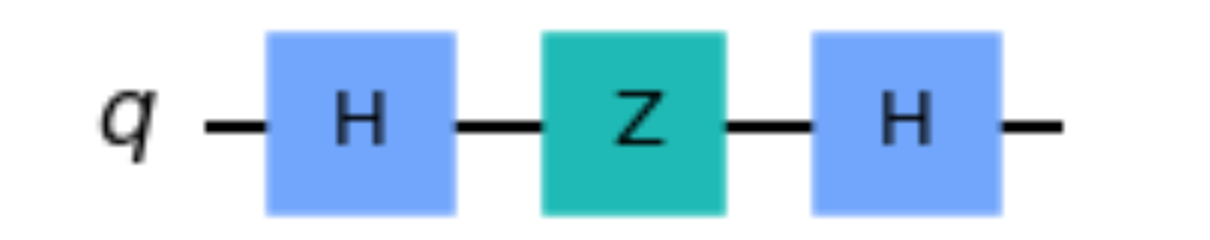
\includegraphics[width=0.4\textwidth]{lab2/images/hzhCircuit.png}
    \caption{Circuit diagram hzh} 
    \label{fig:hzhCircuit}
\end{figure}

Figure \ref{fig:bSphereHZHGate} shows the Bloch Sphere after each gate is applied.

\begin{figure}[h]
    \centering
    \begin{subfigure}[h]{0.24\textwidth}
        \centering
        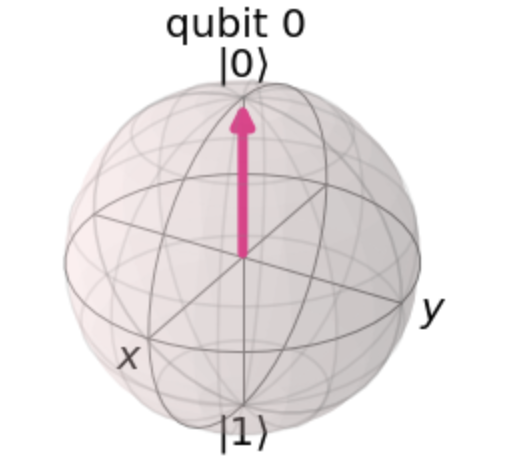
\includegraphics[width=\textwidth]{lab2/images/hzhGate1.png}
        \caption{Initial state}
        \label{fig:hzhGate1}
    \end{subfigure}
    \hfill
    \begin{subfigure}[h]{0.24\textwidth}
        \centering
        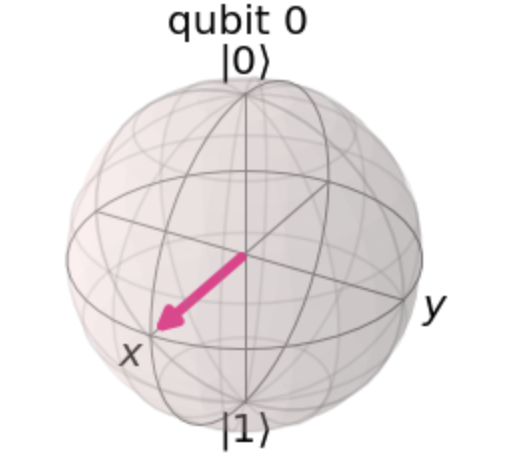
\includegraphics[width=\textwidth]{lab2/images/hzhGate2.png}
        \caption{H gate Applied}
        \label{fig:hzhGate2}
    \end{subfigure}
        \begin{subfigure}[h]{0.24\textwidth}
        \centering
        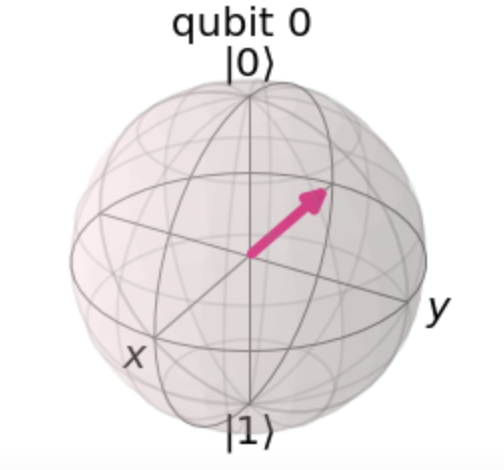
\includegraphics[width=\textwidth]{lab2/images/hzhGate3.png}
        \caption{Z gate applied}
        \label{fig:hzhGate3}
    \end{subfigure}
        \begin{subfigure}[h]{0.24\textwidth}
        \centering
        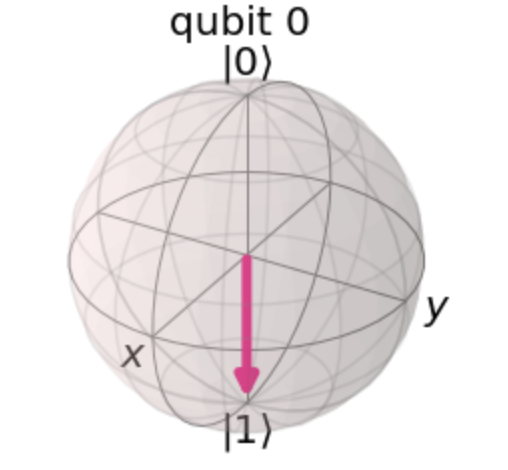
\includegraphics[width=\textwidth]{lab2/images/hzhGate4.png}
        \caption{H gate applied}
        \label{fig:hzhGate4}
    \end{subfigure}
    \caption{Bloch sphere showing qubit state before and after X gate is applied} 
    \label{fig:bSphereHZHGate}
\end{figure}

\subsection{Multi-Qubit Gates}

how to represent the state of a qubit and how to alter those using quantum gates

\subsubsection{Single Qubit Gates on Multi-Qubit Statevectors}

\subsubsection{The CNOT-Gate}
An important two-qubit gate is the CNOT-gate. This gate is a conditional gate that performs an X-gate on the second qubit (target), if the state of the first qubit (control) is  $|1\rangle$

The gate is drawn on a circuit as shwon below, with q\_1 as the control and q\_2 as the target

A 2-qubit quantum circuit was created, where the 2 qubits are entangled and the output was measured. The circuit diagram is shown in Figure \ref{fig:entangleMeasure}

\begin{figure}[h]
    \centering
    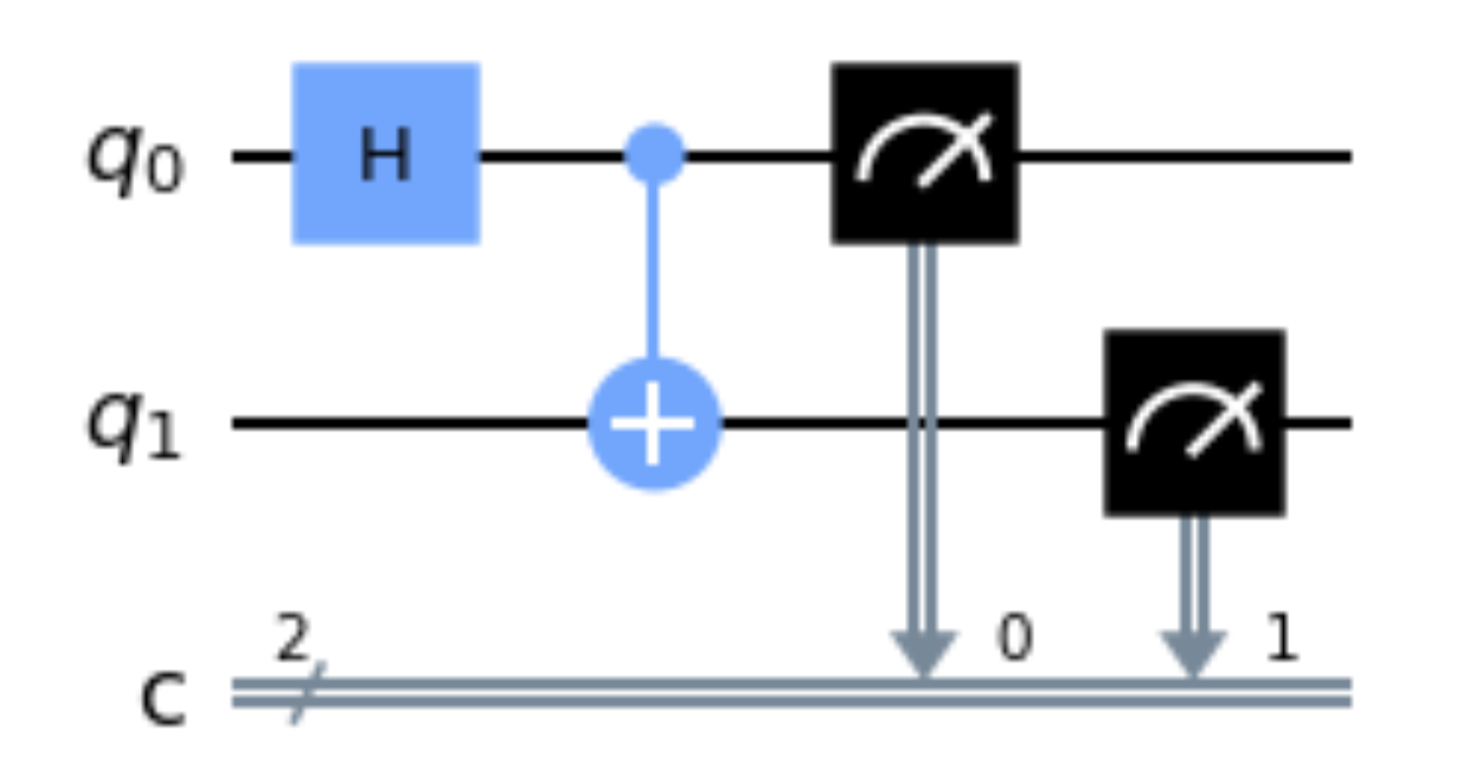
\includegraphics[width=0.4\textwidth]{lab2/images/entangleMeasure.png}
    \caption{entangleMeasure} 
    \label{fig:entangleMeasure}
\end{figure}

The results can be seen in Figure \ref{fig:qiskitHistogram}

\begin{figure}[h]
    \centering
    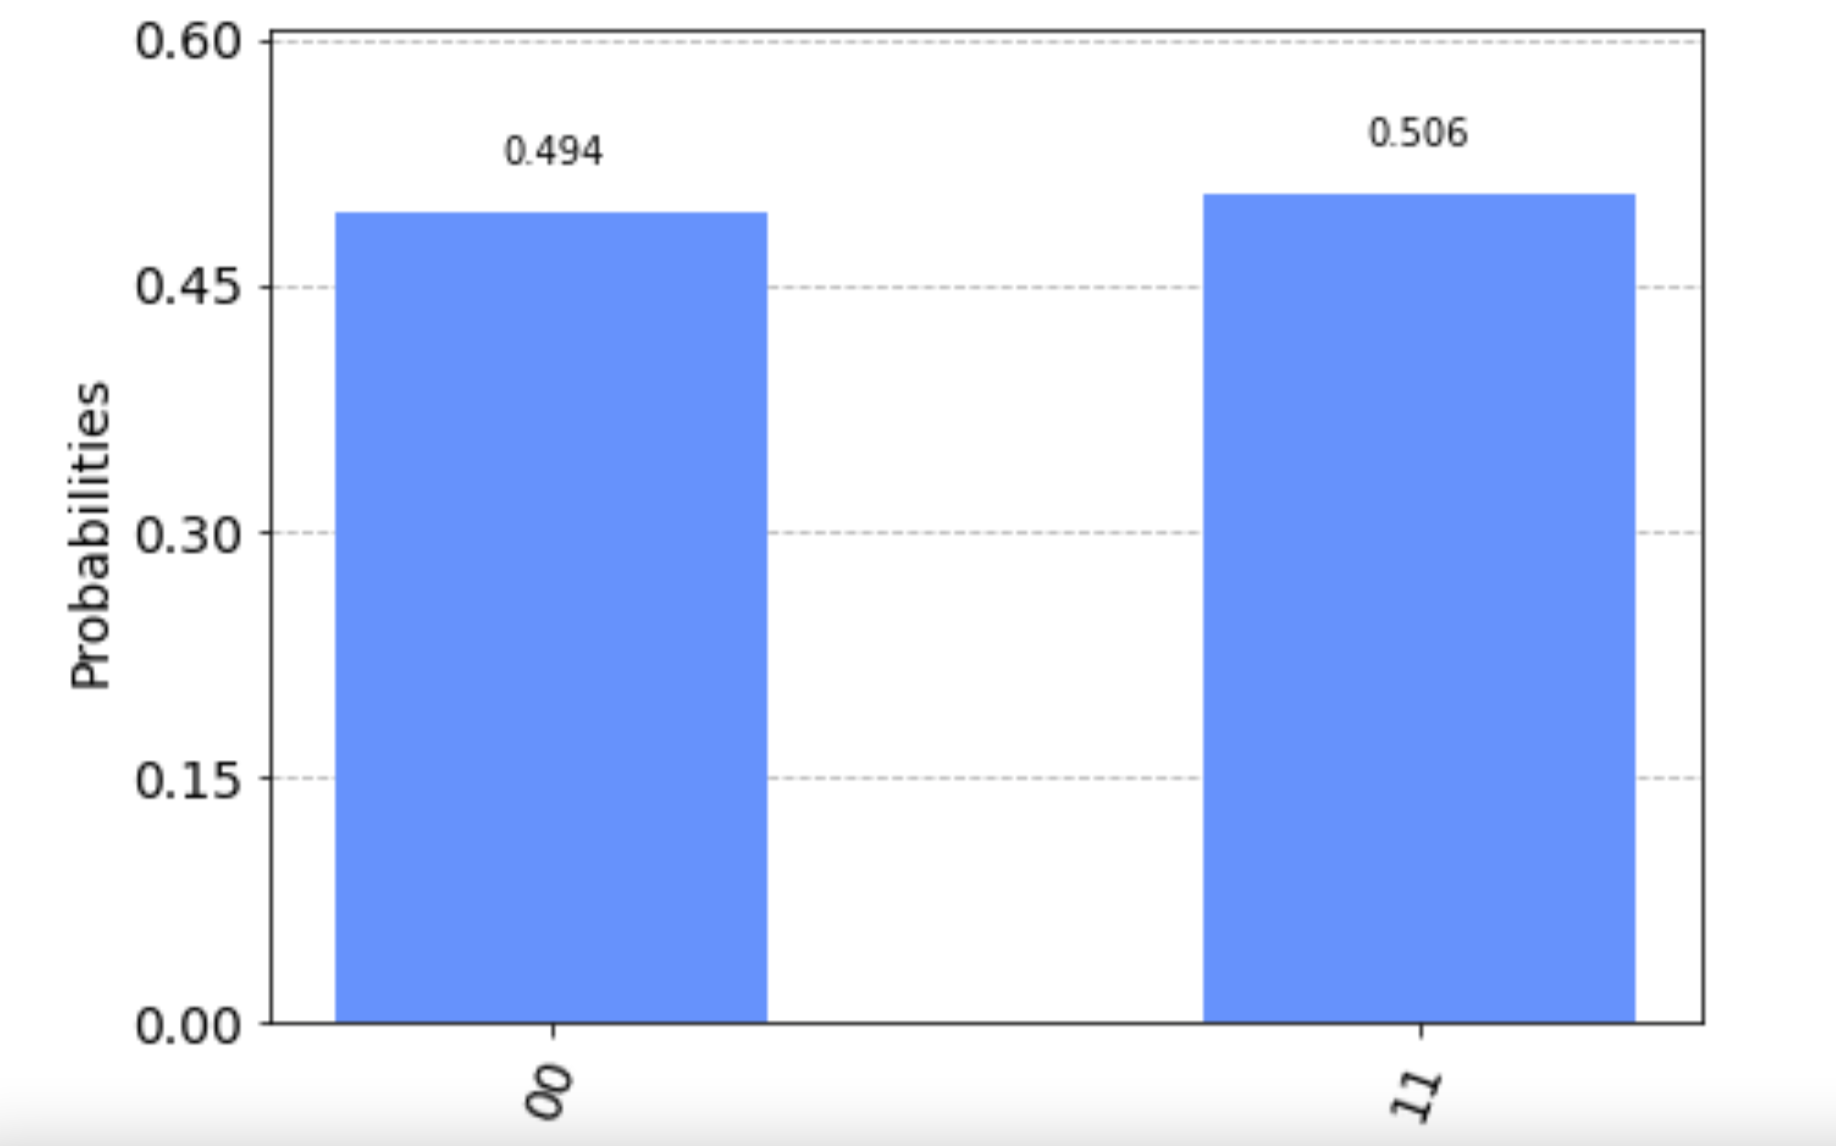
\includegraphics[width=0.75\textwidth]{lab2/images/qiskitHistogram.png}
    \caption{qiskitHistogram} 
    \label{fig:qiskitHistogram}
\end{figure} 

This is different to the theory. Explanation.

\section{Comparison of results with theory}
\section{Discussion}
\textbf{Question 1:}

Initialise a qubit, and apply the X-gate to it. Confirm your result by drawing the circuit and visualing the flipped state using the Block sphere (use/copy and paste the examples above wherever appropriate).


\textbf{Question 2:}
Apply the x and y gates to the qubit above and draw it on your screen.

That is not a question.

\textbf{Question 3:}
Show mathematically that applying the sequence of gates: HZH, to any qubit state is equivalent to applying an X-gate. Then, write a circuit that will show this (you can check each step/rotation, by ploting the new state on the Bloch Sphere each time.


\textbf{Question 4:}
Build a 2-qubit quantum circuit where the 2 qubits are entangled and measure the output. Does this agree with the mathematical prediction? If not, why would you say that is so

\textbf{Question 5:}
Use IBM composer and compare its results to what you obtained above. Are they different? How so? Is there anything you can do to make the results come closer to the mathematica expectation?

\section{Conclusions}